\documentclass[twoside]{article}
\usepackage{graphicx}
\graphicspath{ {./Col_esc_Figures/} }
\usepackage{lipsum} % Package to generate dummy text throughout this template
\usepackage{wrapfig}
\usepackage[sc]{mathpazo} % Use the Palatino font
\usepackage{amsmath}
\usepackage[T1]{fontenc} % Use 8-bit encoding that has 256 glyphs
\linespread{1.50} % Line spacing - Palatino needs more space between lines
\usepackage{microtype} % Slightly tweak font spacing for aesthetics
\usepackage{lineno}
\usepackage{putex}
\usepackage[hmarginratio=1:1,top=32mm,columnsep=20pt]{geometry} % Document margins
\usepackage{multicol} % Used for the two-column layout of the document
\usepackage[hang, small,labelfont=bf,up,textfont=it,up]{caption} % Custom captions under/above floats in tables or figures
\usepackage{booktabs} % Horizontal rules in tables
\usepackage{float} % Required for tables and figures in the multi-column environment - they need to be placed in specific locations with the [H] (e.g. \begin{table}[H])
\usepackage{hyperref} % For hyperlinks in the PDF
\usepackage{lettrine} % The lettrine is the first enlarged letter at the beginning of the text
\usepackage{paralist} % Used for the compactitem environment which makes bullet points with less space between them
\usepackage{enumitem}
\usepackage{mathrsfs}
\setlist[itemize]{noitemsep}  %Remove spacing in lists
\usepackage{abstract} % Allows abstract customization
%\renewcommand{\abstractnamefont}{\normalfont\bfseries} % Set the "Abstract" text to bold
%\renewcommand{\abstracttextfont}{\normalfont\small\itshape} % Set the abstract itself to small italic text
\usepackage{newtxtext,newtxmath}
\usepackage{titlesec} % Allows customization of titles
\renewcommand\thesection{\Roman{section}} % Roman numerals for the sections
\renewcommand\thesubsection{\Roman{subsection}} % Roman numerals for subsections
\titleformat{\section}[block]{\large\scshape\centering}{\thesection.}{1em}{} % Change the look of the section titles
\titleformat{\subsection}[block]{\large}{\thesubsection.}{1em}{} % Change the look of the section titles
\begin{document}
%----------------------------------------------------------------------------------------
%Supplemental Information
%----------------------------------------------------------------------------------------
\subsection*{Supporting Information}
~\\
\textbf{Article title:} The impacts of dew-induced foliar shielding on the energy, water and isotope balance of leaves\\
~\\
\textbf{Authors:} Cynthia Gerlein-Safdi, Craig James Sinkler, Kelly Krispin Caylor\\
~\\
The following Supporting Information is available for this article:\\
\textbf{Fig. \ref{expe1A2H}}: Interpolated maps showing the $\delta$D of the leaves analyzed in Experiment 1A.\\
\textbf{Fig. \ref{expe1A18O}}: Interpolated maps showing the $\delta^{\text{18}}$O of the leaves analyzed in Experiment 1A.\\
%\textbf{Fig. \ref{dewpoint}}: Rainfall amount, air and dew point temperatures for the course of Experiment 1A.

%%%%%%%%%% Merge with supplemental materials %%%%%%%%%%
%%%%%%%%%% Prefix a "S" to all equations, figures, tables and reset the counter %%%%%%%%%%
\setcounter{equation}{0}
\setcounter{figure}{0}
\setcounter{table}{0}
\setcounter{page}{1}
%\makeatletter
\renewcommand{\theequation}{S\arabic{equation}}
\renewcommand{\thefigure}{S\arabic{figure}}

\begin{center}
	\begin{figure}[h!]
		\centering
		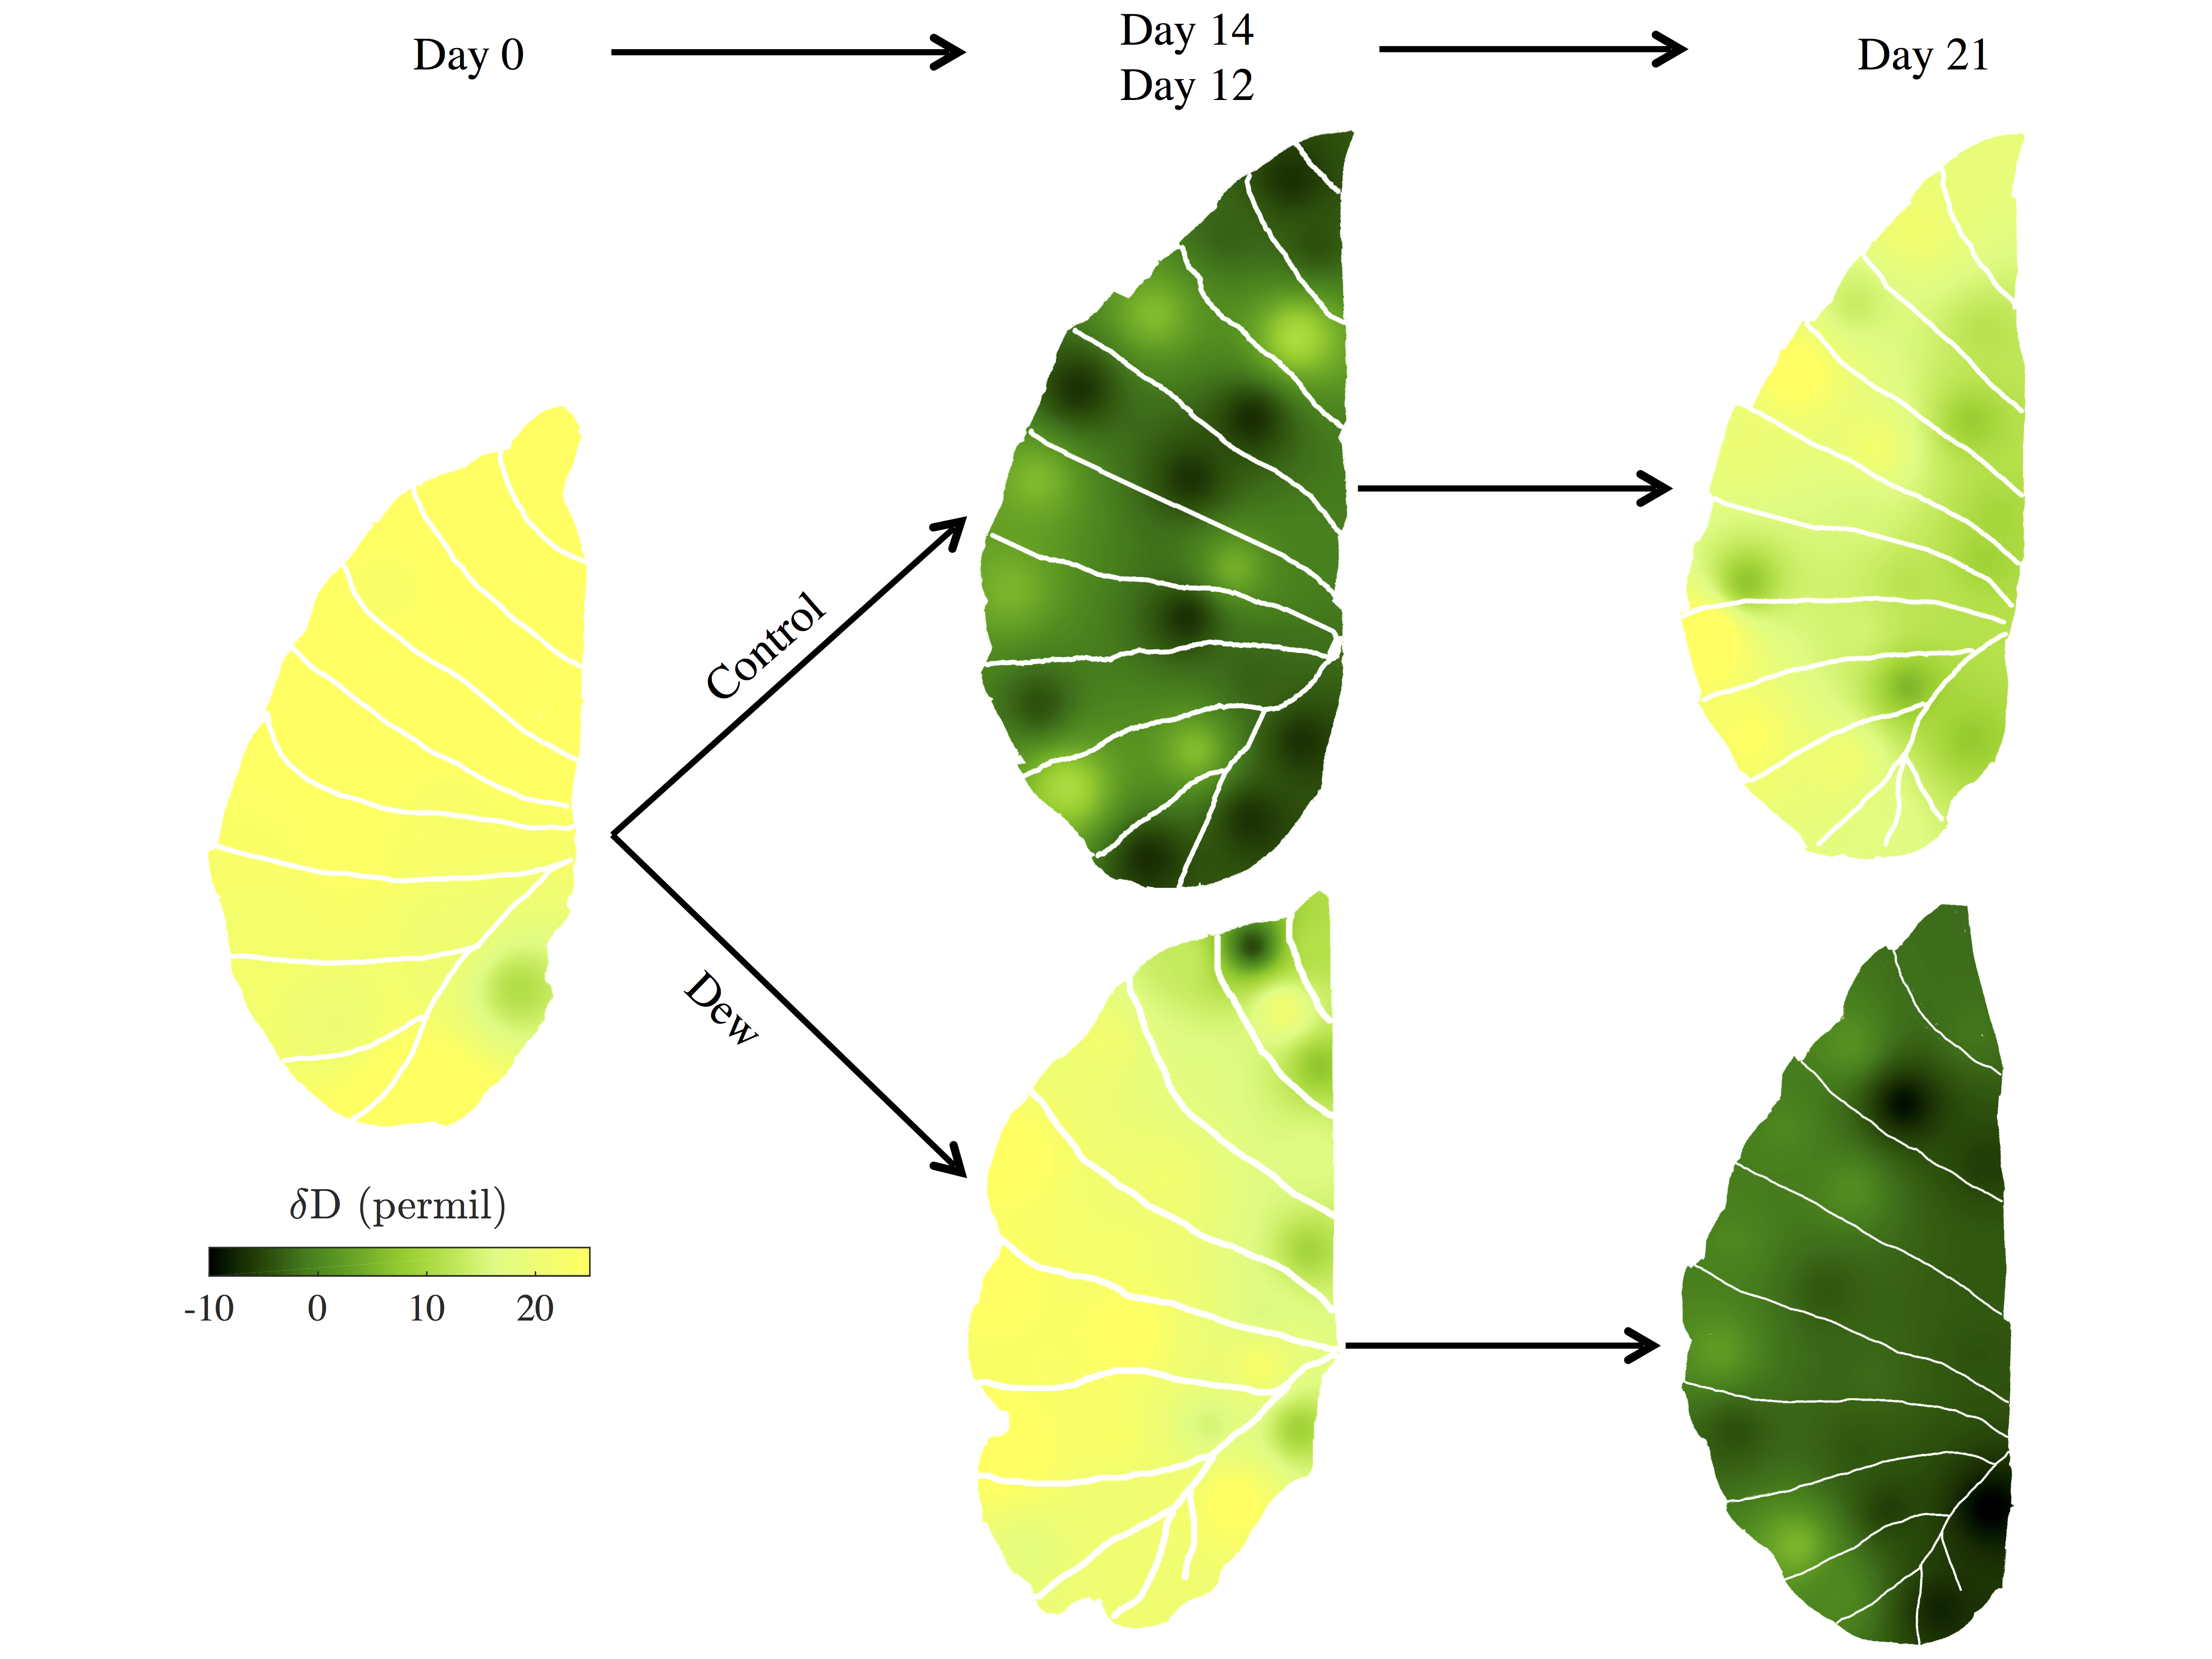
\includegraphics[width=\textwidth]{Final_2H_Plot_GoodQ.jpg}
		\caption{Maps of the spacial distribution of $\delta$D of five \textit{Colocasia esculenta} leaves collected throughout Experiment 1A. The maps were obtained by inverse distance interpolation of 12 to 25 sampling points analyzed on the Picarro Induction Module. All leaves are c. 38~cm long. \textbf{Left:} initial leaf collected on day 0. \textbf{Top row:} leaves collected on day 14 (center) and 21 (far right) from the control. \textbf{Bottom row:} leaves collected on day 12 (center) and 21 (far right) from the sprayed treatment, where the leaves were sprayed with isotopically enriched water ($\delta^{18}$O~$\simeq$~8.85~\textperthousand, $\delta$D~$\simeq$~737.64~\textperthousand) every two days. The color scheme is the same for all rows.}\label{expe1A2H}
	\end{figure}
\end{center}
\begin{center}
	\begin{figure}[h!]
		\centering
		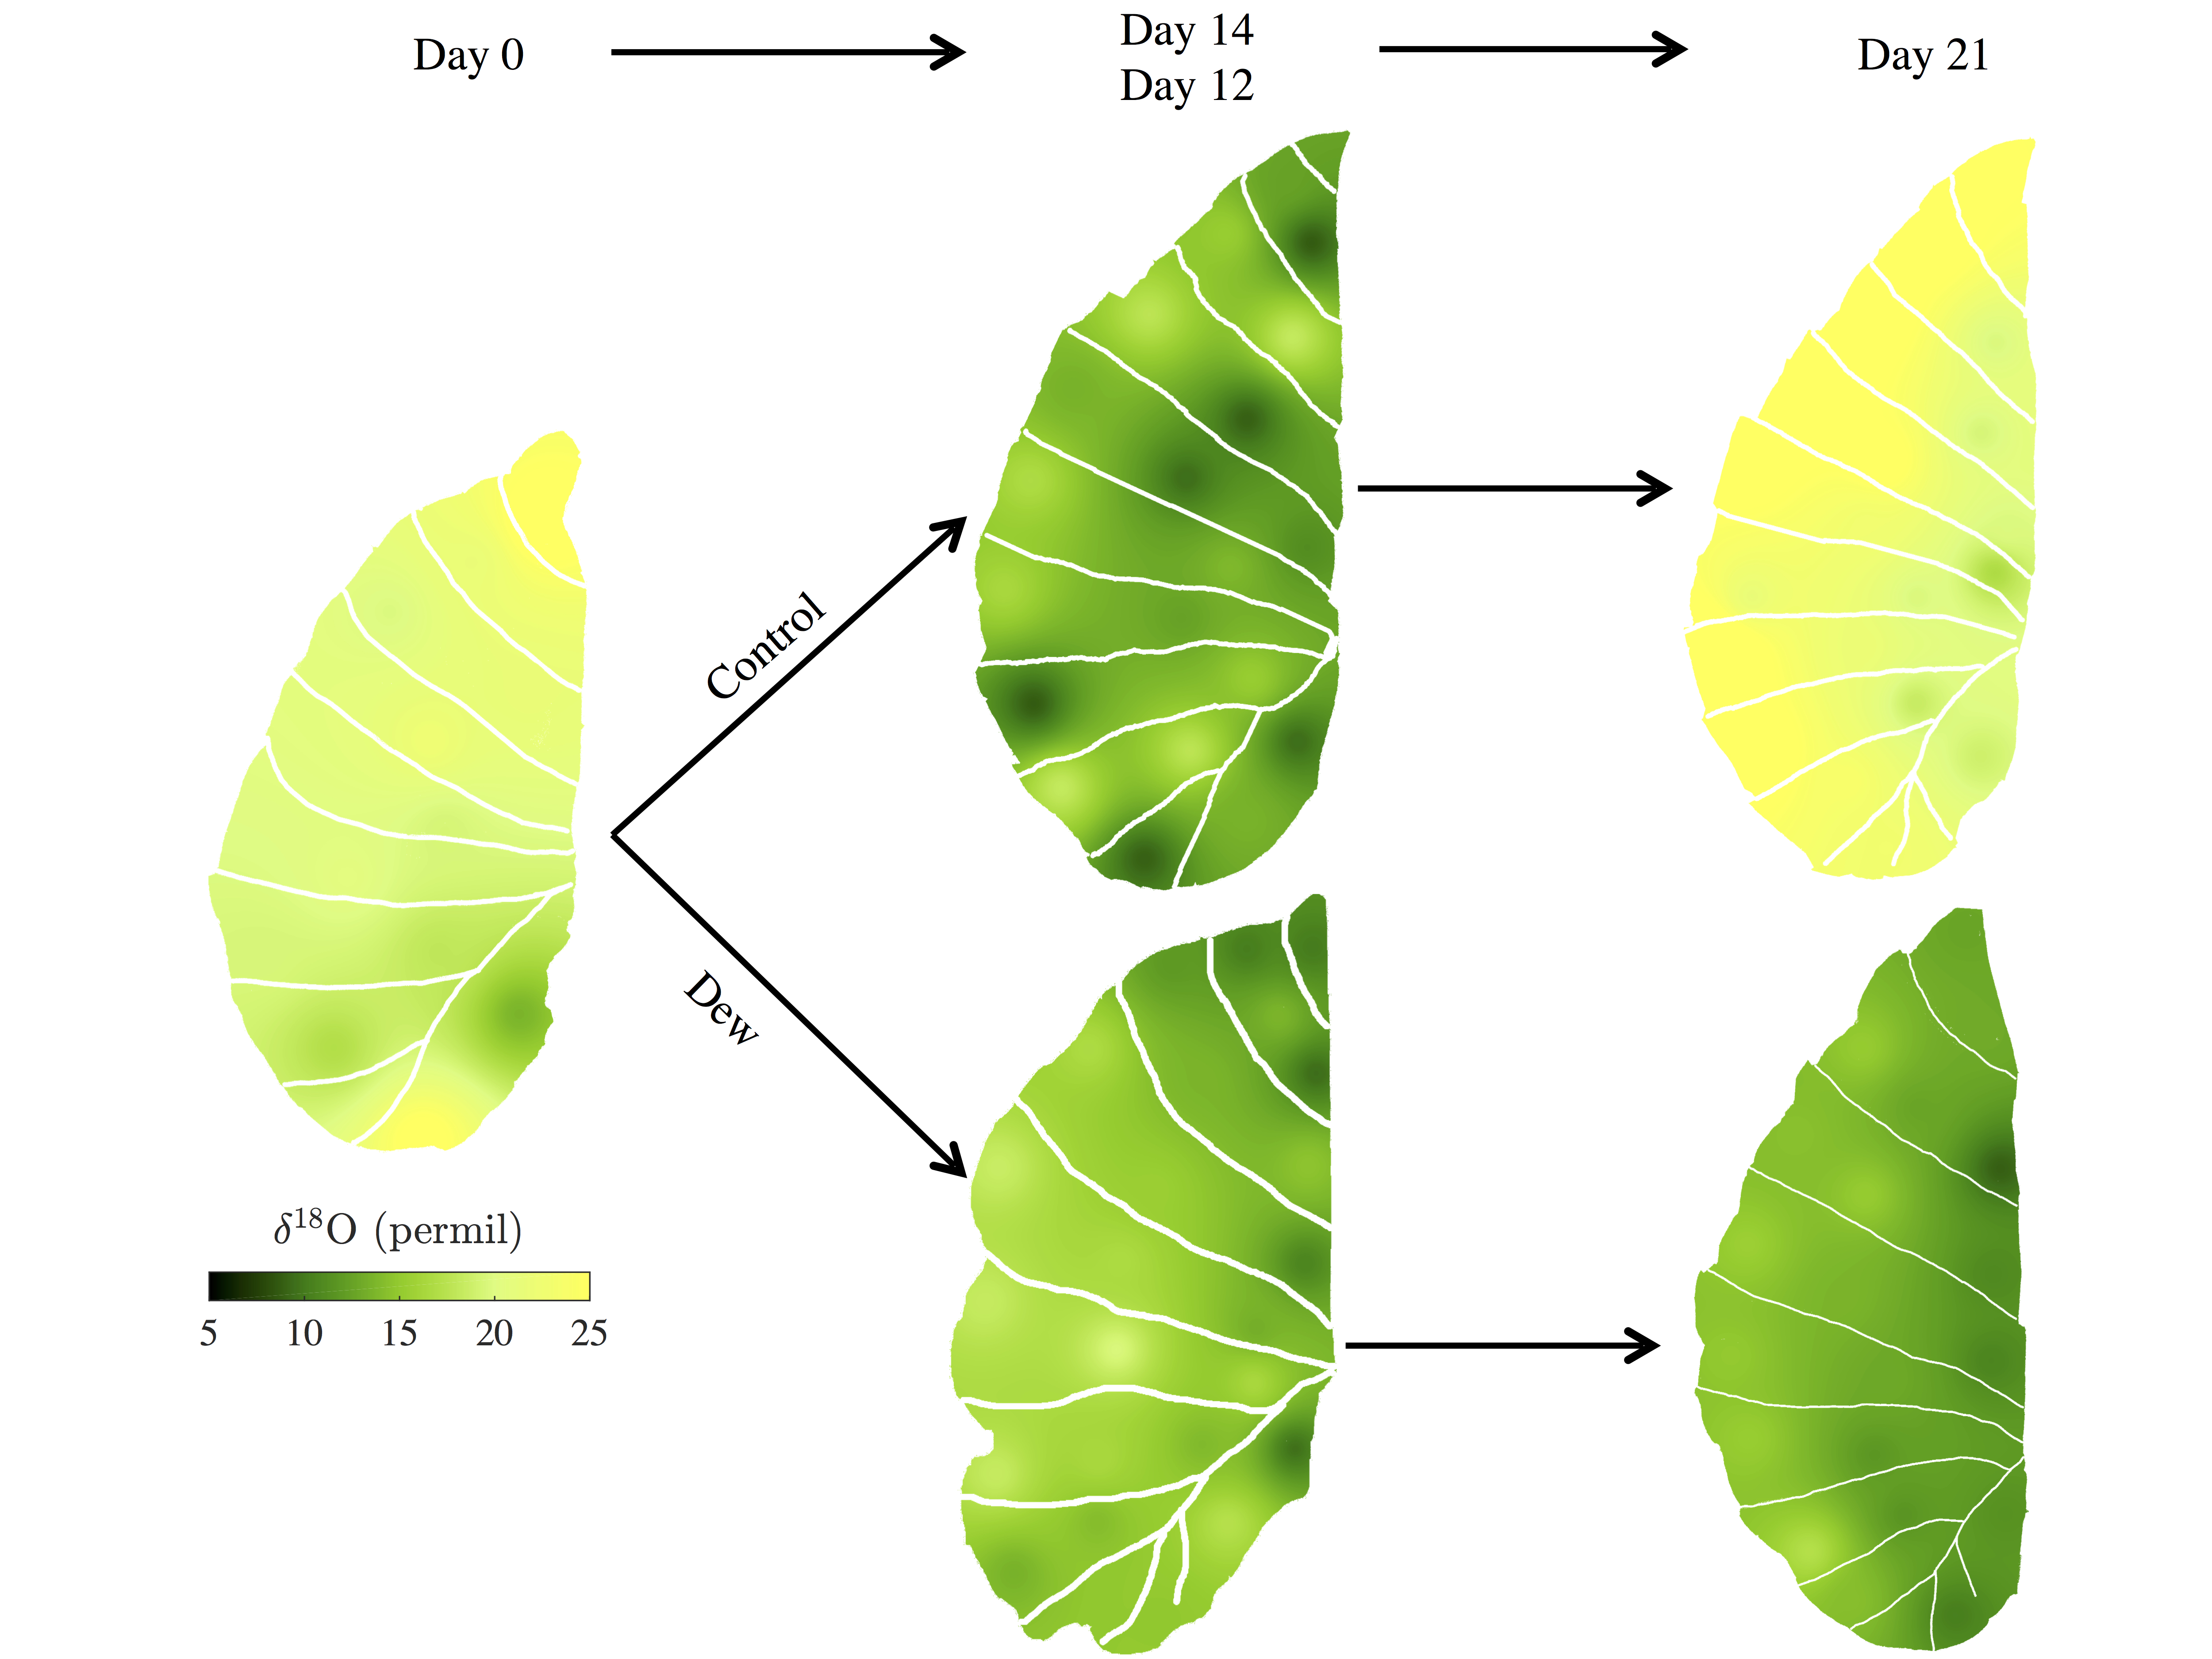
\includegraphics[width=\textwidth]{Final_18O_Plot_GoodQ.jpg}
		\caption{Maps of the spacial distribution of $\delta^{\text{18}}$O of five \textit{Colocasia esculenta} leaves collected throughout Experiment 1A. The maps were obtained by inverse distance interpolation of 12 to 25 sampling points analyzed on the Picarro Induction Module. All leaves are c. 38~cm long. \textbf{Left:} initial leaf collected on day 0. \textbf{Top row:} leaves collected on day 14 (center) and 21 (far right) from the control. \textbf{Bottom row:} leaves collected on day 12 (center) and 21 (far right) from the sprayed treatment, where the leaves were sprayed with isotopically enriched water ($\delta^{18}$O~$\simeq$~8.85~\textperthousand, $\delta$D~$\simeq$~737.64~\textperthousand) every two days. The color scheme is the same for all rows.}\label{expe1A18O}
	\end{figure}
\end{center}
%\begin{center}
%	\begin{figure}
%		\centering
%		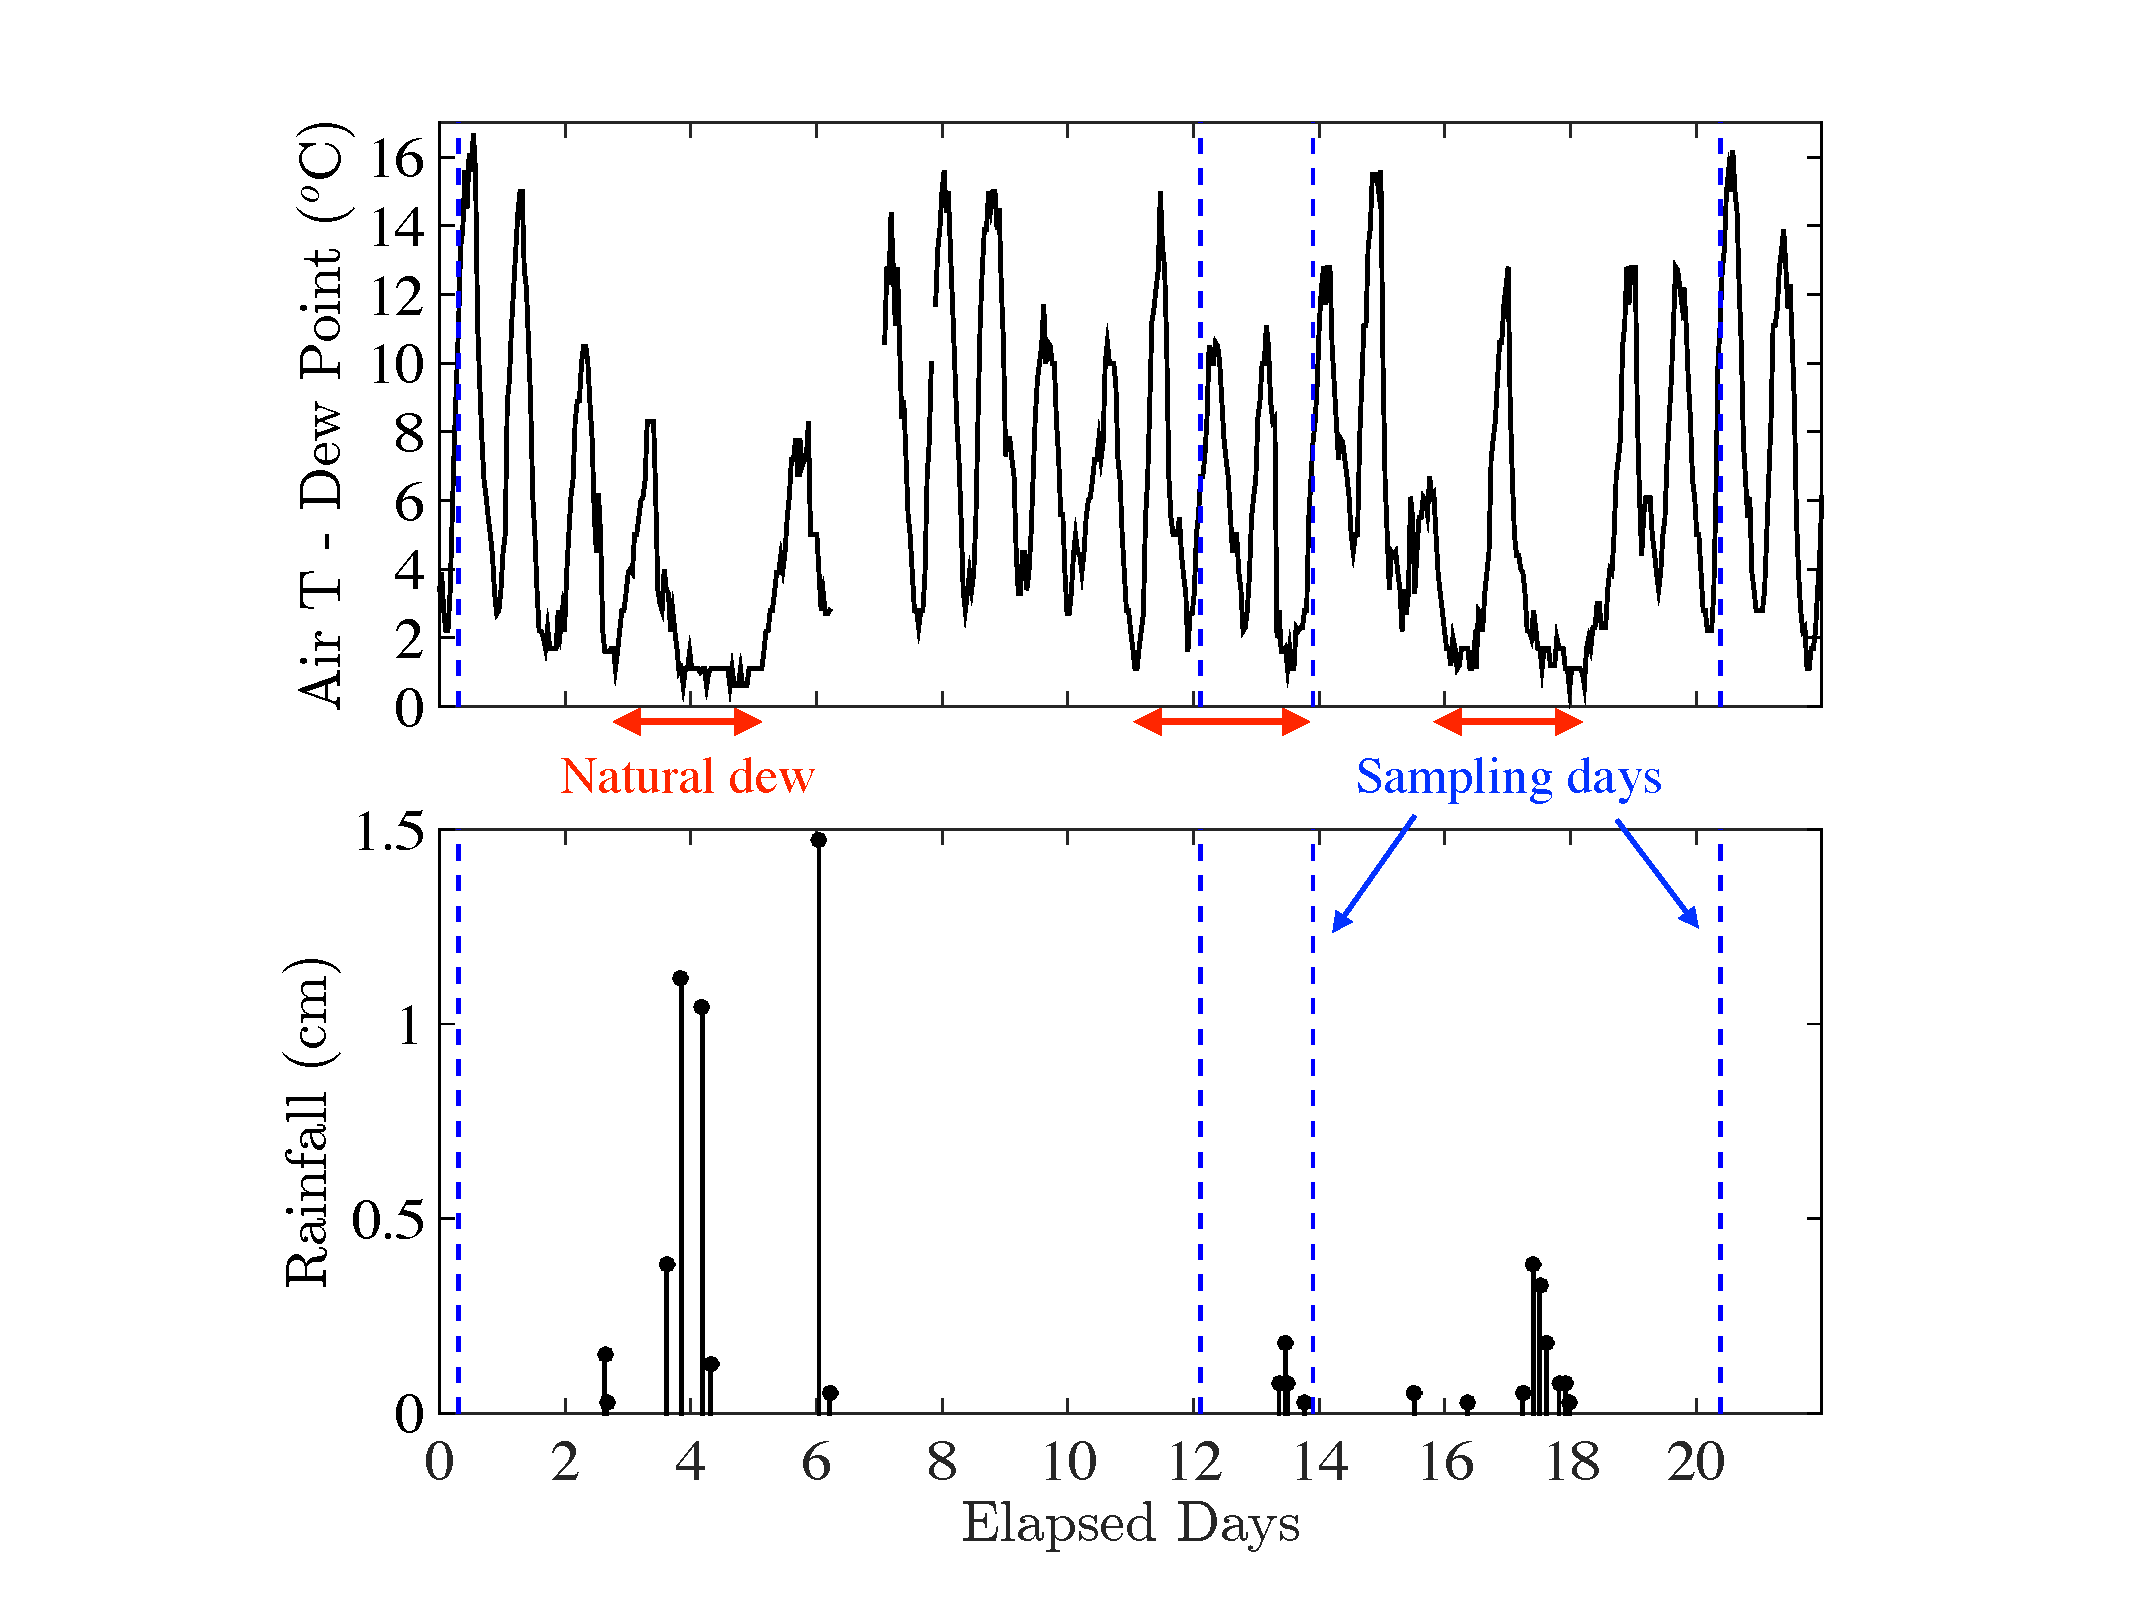
\includegraphics[width=0.8\textwidth]{Experiment_DewPoint_T_Annotated.pdf}
%		\caption{\textbf{Top panel:} Difference between the air and the dew point temperature over the course of the experiment ($^{\text{o}}$C). \textbf{Bottom panel:} Rainfall (cm) over the course of the experiment. The blue dashed vertical lines mark the days of collection: the initial leaf was collected on day 0, leaves from the dew treatment were collected on days 12 and 21 and leaves from the control were collected on days 14 and 21. Red horizontal arrows indicate days when the leaves most likely experienced natural dew deposition because of the local air temperature and relative humidity under the sheltered area. The collection of the first control leaf happened after a series of small rain events and four nights of natural dew formation.}\label{dewpoint}
%	\end{figure}
%\end{center}
\end{document}
